\documentclass[11pt,a4paper]{article}
\usepackage[utf8]{inputenc}
\usepackage[margin=1in]{geometry}
\usepackage{amsmath, amssymb}
\usepackage{tikz}
\usetikzlibrary{shapes.geometric, arrows.meta, positioning, calc, fit, backgrounds, decorations.pathmorphing}
\usepackage{caption}
\usepackage{subcaption}

% =========================================================================
% NVIDIA BRAND COLOR PALETTE (Figure 1)
% =========================================================================
\definecolor{nvidiagreen}{RGB}{118, 185, 0}    % NVIDIA Signature Green (#76B900)
\definecolor{nvidiadark}{RGB}{26, 59, 5}       % Deep Forest Green (#1A3B05)
\definecolor{nvidiablack}{RGB}{17, 24, 15}     % Sleek Tech Charcoal
\definecolor{nvidiabg}{RGB}{248, 251, 244}     % Ultra-clean Pale Mint-Gray
\definecolor{cardborder}{RGB}{95, 150, 2}      % Refined Accent Green Border

\definecolor{attnfill}{RGB}{232, 246, 212}     % Soft Green for Attention
\definecolor{ffnfill}{RGB}{214, 240, 184}      % Mid Green for SwiGLU FFN
\definecolor{normfill}{RGB}{244, 250, 235}     % Pale Mint for RMSNorm / Add
\definecolor{embedfill}{RGB}{237, 247, 225}    % Light Sage for Token Embed
\definecolor{charfill}{RGB}{225, 242, 203}     % Soft Green-Sage for Char-CNN
\definecolor{headfill}{RGB}{118, 185, 0}       % Bold NVIDIA Green for Heads
\definecolor{ropefill}{RGB}{156, 229, 20}      % Bright Lime Accent for RoPE
\definecolor{bannerfill}{RGB}{26, 59, 5}       % Dark Emerald for Task Banners

% Classic Vaswani Palette (Figure 2)
\definecolor{vas_attn}{RGB}{255, 229, 180}
\definecolor{vas_ffn}{RGB}{207, 226, 243}
\definecolor{vas_norm}{RGB}{255, 242, 204}
\definecolor{vas_embed}{RGB}{244, 204, 204}
\definecolor{vas_linear}{RGB}{217, 210, 233}
\definecolor{vas_softmax}{RGB}{217, 234, 211}
\definecolor{vas_bg}{RGB}{245, 245, 247}
\definecolor{vas_pos}{RGB}{255, 217, 102}

\tikzset{
    box/.style={
        draw=cardborder,
        line width=1.1pt,
        rounded corners=5pt,
        font=\sffamily\footnotesize,
        text centered,
        align=center,
        inner sep=4pt,
        text=nvidiablack
    },
    attn/.style={box, fill=attnfill, minimum height=0.80cm, minimum width=3.8cm},
    ffn/.style={box, fill=ffnfill, minimum height=0.80cm, minimum width=3.8cm},
    norm/.style={box, fill=normfill, minimum height=0.68cm, minimum width=3.8cm},
    embed/.style={box, fill=embedfill, minimum height=0.85cm, minimum width=3.2cm},
    charcnn/.style={box, fill=charfill, minimum height=0.85cm, minimum width=3.2cm},
    headlinear/.style={
        box,
        draw=nvidiadark,
        fill=normfill,
        line width=1.1pt,
        minimum height=0.78cm,
        minimum width=3.2cm,
        font=\sffamily\bfseries\footnotesize
    },
    headsoftmax/.style={
        box,
        draw=nvidiadark,
        fill=headfill,
        line width=1.1pt,
        minimum height=0.68cm,
        minimum width=3.2cm,
        font=\sffamily\bfseries\footnotesize,
        text=white
    },
    taskbanner/.style={
        draw=nvidiadark,
        line width=1.0pt,
        fill=bannerfill,
        rounded corners=3pt,
        font=\sffamily\bfseries\scriptsize,
        text=white,
        inner sep=3.5pt,
        minimum width=3.2cm,
        text centered,
        align=center
    },
    addcircle/.style={
        circle,
        draw=nvidiadark,
        line width=1.1pt,
        fill=white,
        inner sep=0pt,
        minimum size=0.52cm,
        font=\bfseries\normalsize,
        text=nvidiadark
    },
    arrow/.style={
        -{Stealth[scale=1.15]},
        line width=1.1pt,
        draw=nvidiadark
    },
    line/.style={
        line width=1.1pt,
        draw=nvidiadark
    },
    textlabel/.style={
        font=\sffamily\footnotesize,
        text centered,
        align=center,
        text=nvidiablack
    }
}

\begin{document}

\title{\textbf{TypoFormer Model Architecture Specification}}
\author{Md. Fahim Sarker Mridul}
\date{\today}
\maketitle

\section{TypoFormer Architecture Diagram (NVIDIA Green Theme)}
Below is the complete internal architecture of the \textbf{TypoFormer} keystroke companion, featuring dual-channel character-aware token fusion, pre-norm grouped-query attention with rotary embeddings (RoPE), SwiGLU feed-forward networks, and multi-task heads for real-time autocomplete and grammar error correction.

\begin{figure}[htbp]
\centering
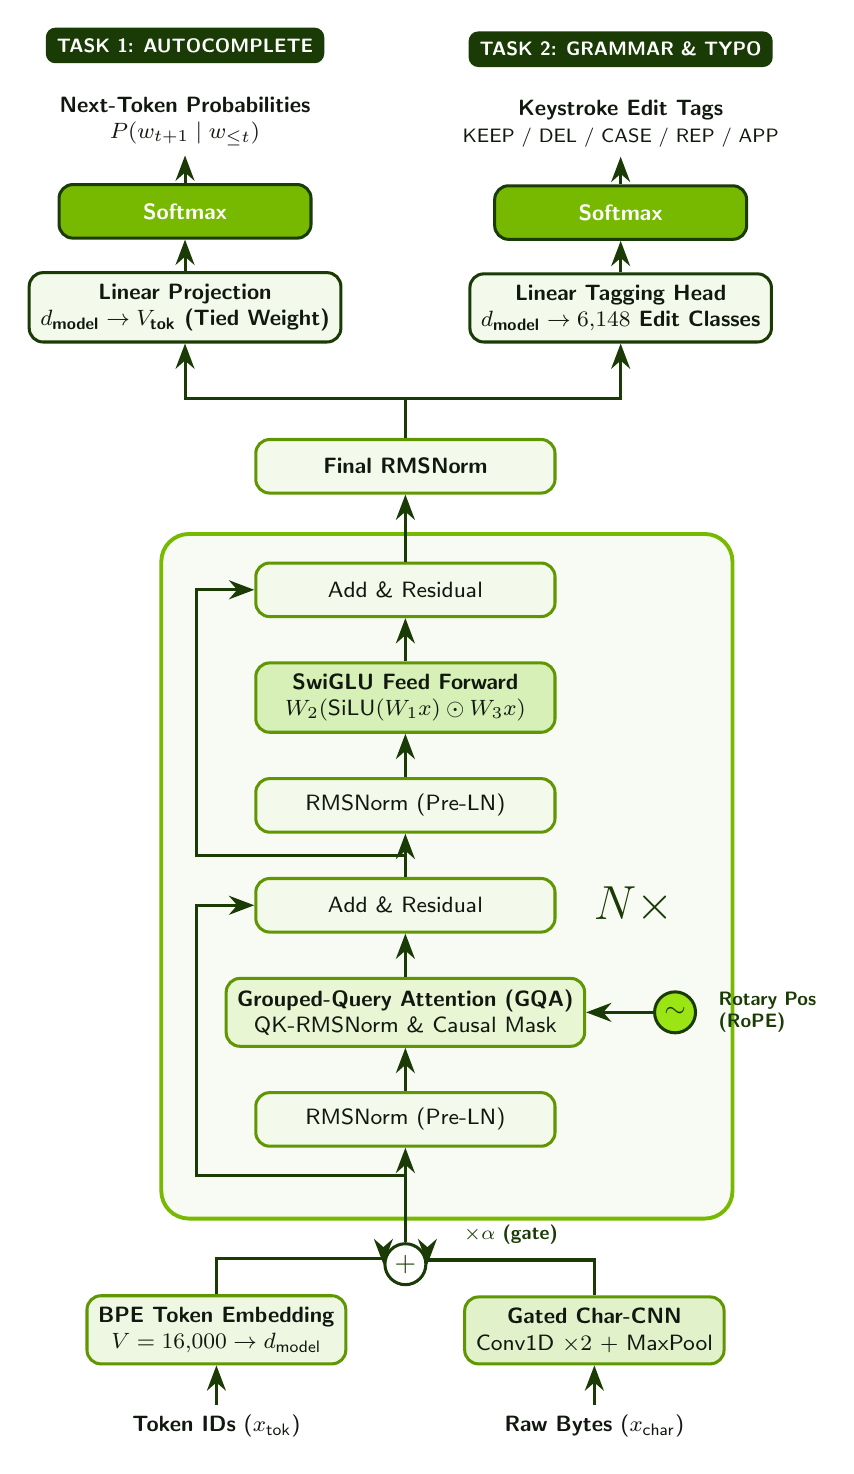
\begin{tikzpicture}[node distance=0.65cm and 1.0cm]

    % --- 1. BOTTOM INPUTS & DUAL EMBEDDINGS ---
    \node[textlabel] (tok_in) at (-2.4, 0) {\textbf{Token IDs} ($x_{\text{tok}}$)};
    \node[textlabel] (char_in) at (2.4, 0) {\textbf{Raw Bytes} ($x_{\text{char}}$)};

    \node[embed, above=0.5cm of tok_in] (tok_emb) {\textbf{BPE Token Embedding}\\$V = 16{,}000 \to d_{\text{model}}$};
    \node[charcnn, above=0.5cm of char_in] (char_emb) {\textbf{Gated Char-CNN}\\Conv1D $\times 2$ + MaxPool};

    \draw[arrow] (tok_in) -- (tok_emb);
    \draw[arrow] (char_in) -- (char_emb);

    % Fused Addition Node (+)
    \node[addcircle] (fuse_add) at (0, 2.05) {$+$};

    \draw[arrow] (tok_emb.north) -- ++(0, 0.45cm) -| (fuse_add.west);
    
    \coordinate (char_corner) at ($(char_emb.north) + (0, 0.45cm)$);
    \draw[arrow] (char_emb.north) -- (char_corner) -| (fuse_add.east);
    
    \node[font=\sffamily\bfseries\scriptsize, text=nvidiadark, above=2pt] at ($(char_corner)!0.5!(char_corner -| fuse_add.east)$) {$\times \alpha \text{ (gate)}$};

    % --- 2. TRANSFORMER BACKBONE (Nx BLOCK) ---
    \node[norm, above=1.2cm of fuse_add] (norm1) {RMSNorm (Pre-LN)};
    \draw[arrow] (fuse_add) -- (norm1);

    \node[attn, above=0.55cm of norm1] (attn) {\textbf{Grouped-Query Attention (GQA)}\\QK-RMSNorm \& Causal Mask};
    \draw[arrow] (norm1) -- (attn);

    \node[addcircle, right=0.85cm of attn, fill=ropefill] (rope_icon) {$\sim$};
    \node[textlabel, right=0.15cm of rope_icon, align=left, font=\sffamily\scriptsize\bfseries, text=nvidiadark] {Rotary Pos\\(RoPE)};
    \draw[arrow] (rope_icon) -- (attn.east);

    \node[norm, above=0.55cm of attn] (add1) {Add \& Residual};
    \draw[arrow] (attn) -- (add1);

    \coordinate (res1_branch) at ($(norm1.south) + (0, -0.35cm)$);
    \draw[arrow] (res1_branch) -- ++(-2.65cm, 0) |- (add1.west);

    \node[norm, above=0.55cm of add1] (norm2) {RMSNorm (Pre-LN)};
    \draw[arrow] (add1) -- (norm2);

    \node[ffn, above=0.55cm of norm2] (ffn) {\textbf{SwiGLU Feed Forward}\\$W_2(\text{SiLU}(W_1 x) \odot W_3 x)$};
    \draw[arrow] (norm2) -- (ffn);

    \node[norm, above=0.55cm of ffn] (add2) {Add \& Residual};
    \draw[arrow] (ffn) -- (add2);

    \coordinate (res2_branch) at ($(norm2.south)!0.5!(add1.north)$);
    \draw[arrow] (res2_branch) -- ++(-2.65cm, 0) |- (add2.west);

    \begin{scope}[on background layer]
        \node[
            draw=nvidiagreen,
            line width=1.4pt,
            rounded corners=10pt,
            fill=nvidiabg,
            fit={(norm1) (attn) (add1) (norm2) (ffn) (add2) (rope_icon) ($(res1_branch) + (-2.65cm, -0.2cm)$)},
            inner xsep=0.45cm,
            inner ysep=0.35cm
        ] (nx_box) {};
    \end{scope}

    \node[textlabel, right=0.35cm of add1.east, font=\sffamily\bfseries\LARGE, text=nvidiadark] (nx_label) {$N\times$};

    \node[norm, above=0.85cm of add2] (final_norm) {\textbf{Final RMSNorm}};
    \draw[arrow] (add2) -- (final_norm);

    % --- 3. DUAL MULTI-TASK OUTPUT HEADS ---
    \coordinate (head_split) at ($(final_norm.north) + (0, 0.5cm)$);
    \draw[line] (final_norm.north) -- (head_split);

    \node[headlinear, above left=0.7cm and 0.8cm of head_split] (lm_linear) {\textbf{Linear Projection}\\$d_{\text{model}} \to V_{\text{tok}}$ (Tied Weight)};
    \node[headsoftmax, above=0.4cm of lm_linear] (lm_softmax) {Softmax};
    \node[textlabel, above=0.35cm of lm_softmax, align=center] (lm_out) {\textbf{Next-Token Probabilities}\\$P(w_{t+1} \mid w_{\le t})$};
    \node[taskbanner, above=0.3cm of lm_out] (banner1) {TASK 1: AUTOCOMPLETE};

    \draw[arrow] (head_split) -| (lm_linear.south);
    \draw[arrow] (lm_linear) -- (lm_softmax);
    \draw[arrow] (lm_softmax) -- (lm_out);

    \node[headlinear, above right=0.7cm and 0.8cm of head_split] (gec_linear) {\textbf{Linear Tagging Head}\\$d_{\text{model}} \to 6{,}148\text{ Edit Classes}$};
    \node[headsoftmax, above=0.4cm of gec_linear] (gec_softmax) {Softmax};
    \node[textlabel, above=0.35cm of gec_softmax, align=center] (gec_out) {\textbf{Keystroke Edit Tags}\\{\scriptsize KEEP / DEL / CASE / REP / APP}};
    \node[taskbanner, above=0.3cm of gec_out] (banner2) {TASK 2: GRAMMAR \& TYPO};

    \draw[arrow] (head_split) -| (gec_linear.south);
    \draw[arrow] (gec_linear) -- (gec_softmax);
    \draw[arrow] (gec_softmax) -- (gec_out);

\end{tikzpicture}
\caption{TypoFormer Model Architecture (NVIDIA Green Style): Integrating byte-level subwords with multi-scale character convolutions, pre-norm grouped-query attention, rotary embeddings (RoPE), and joint dual heads for autocomplete and grammar error correction.}
\label{fig:typoformer}
\end{figure}

\newpage
\section{Classic Transformer Architecture (Vaswani et al., 2017)}
For reference and comparison, the exact encoder-decoder architecture from \textit{Attention Is All You Need} is also provided below with identical color grading and geometry.

\begin{figure}[htbp]
\centering
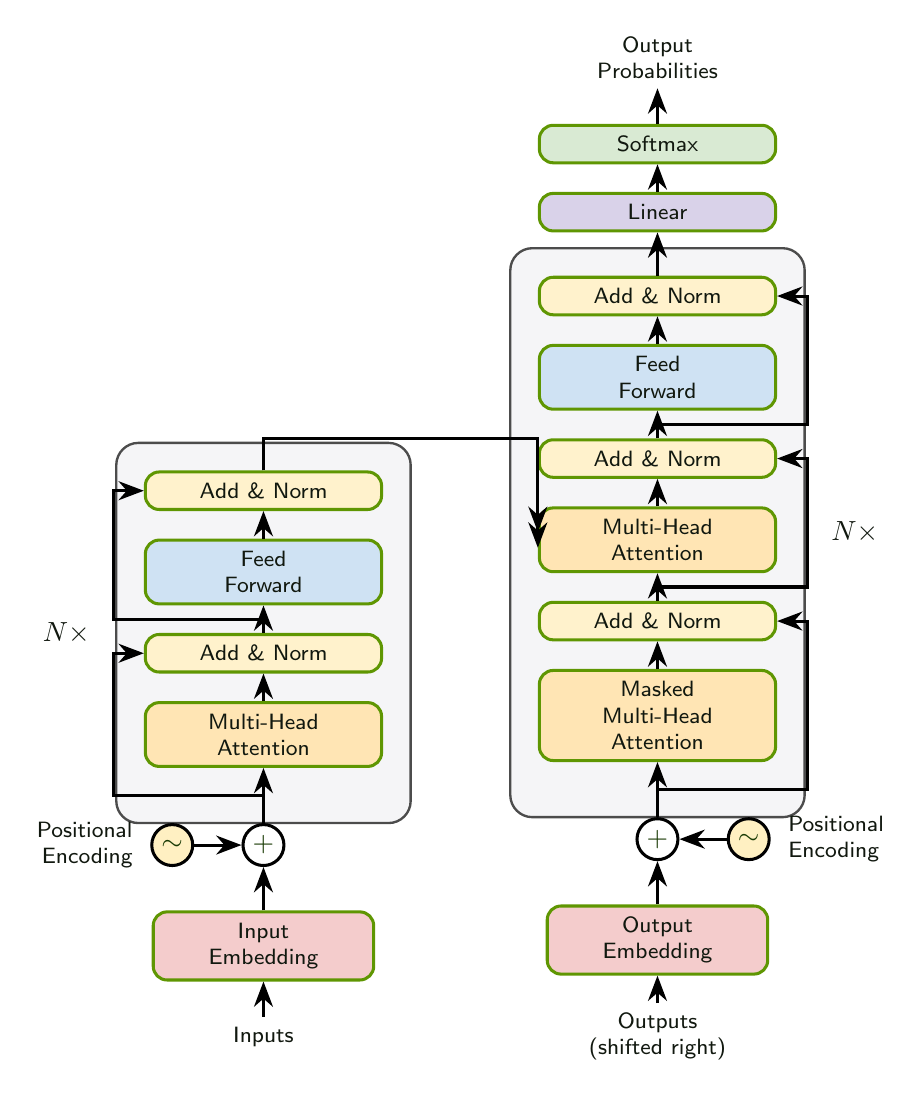
\begin{tikzpicture}[node distance=0.45cm and 0.7cm]

    % ================= ENCODER (LEFT) =================
    \node[textlabel] (enc_in) {Inputs};
    \node[box, fill=vas_embed, above=0.45cm of enc_in, minimum width=2.8cm] (enc_emb) {Input\\Embedding};
    \node[addcircle, draw=black, above=0.55cm of enc_emb] (enc_add0) {$+$};
    \node[addcircle, draw=black, left=0.6cm of enc_add0, fill=vas_pos!40] (enc_pos) {$\sim$};
    \node[textlabel, left=0.1cm of enc_pos, align=right] {Positional\\Encoding};

    \draw[arrow, draw=black] (enc_in) -- (enc_emb);
    \draw[arrow, draw=black] (enc_emb) -- (enc_add0);
    \draw[arrow, draw=black] (enc_pos) -- (enc_add0);

    % Encoder Layers
    \node[box, fill=vas_attn, above=0.7cm of enc_add0, minimum width=3.0cm] (enc_mha) {Multi-Head\\Attention};
    \node[box, fill=vas_norm, above=0.35cm of enc_mha, minimum width=3.0cm] (enc_norm1) {Add \& Norm};
    \node[box, fill=vas_ffn, above=0.35cm of enc_norm1, minimum width=3.0cm] (enc_ffn) {Feed\\Forward};
    \node[box, fill=vas_norm, above=0.35cm of enc_ffn, minimum width=3.0cm] (enc_norm2) {Add \& Norm};

    \draw[arrow, draw=black] (enc_add0) -- (enc_mha);
    \draw[arrow, draw=black] (enc_mha) -- (enc_norm1);
    \draw[arrow, draw=black] (enc_norm1) -- (enc_ffn);
    \draw[arrow, draw=black] (enc_ffn) -- (enc_norm2);

    % Encoder Residuals
    \coordinate (enc_res1) at ($(enc_add0.north)!0.5!(enc_mha.south)$);
    \draw[arrow, draw=black] (enc_res1) -- ++(-1.9cm, 0) |- (enc_norm1.west);

    \coordinate (enc_res2) at ($(enc_norm1.north)!0.5!(enc_ffn.south)$);
    \draw[arrow, draw=black] (enc_res2) -- ++(-1.9cm, 0) |- (enc_norm2.west);

    % Encoder Nx Container
    \begin{scope}[on background layer]
        \node[
            draw=black!70,
            line width=0.85pt,
            rounded corners=8pt,
            fill=vas_bg,
            fit={(enc_res1) (enc_mha) (enc_norm1) (enc_ffn) (enc_norm2)},
            inner xsep=0.35cm,
            inner ysep=0.35cm
        ] (enc_box) {};
    \end{scope}
    \node[textlabel, left=0.2cm of enc_box.west, font=\sffamily\bfseries\normalsize] {$N\times$};

    % ================= DECODER (RIGHT) =================
    \node[textlabel, right=3.5cm of enc_in] (dec_in) {Outputs\\(shifted right)};
    \node[box, fill=vas_embed, above=0.35cm of dec_in, minimum width=2.8cm] (dec_emb) {Output\\Embedding};
    \node[addcircle, draw=black, above=0.55cm of dec_emb] (dec_add0) {$+$};
    \node[addcircle, draw=black, right=0.6cm of dec_add0, fill=vas_pos!40] (dec_pos) {$\sim$};
    \node[textlabel, right=0.1cm of dec_pos, align=left] {Positional\\Encoding};

    \draw[arrow, draw=black] (dec_in) -- (dec_emb);
    \draw[arrow, draw=black] (dec_emb) -- (dec_add0);
    \draw[arrow, draw=black] (dec_pos) -- (dec_add0);

    % Decoder Layers
    \node[box, fill=vas_attn, above=0.7cm of dec_add0, minimum width=3.0cm] (dec_mask_mha) {Masked\\Multi-Head\\Attention};
    \node[box, fill=vas_norm, above=0.35cm of dec_mask_mha, minimum width=3.0cm] (dec_norm1) {Add \& Norm};
    \node[box, fill=vas_attn, above=0.35cm of dec_norm1, minimum width=3.0cm] (dec_cross_mha) {Multi-Head\\Attention};
    \node[box, fill=vas_norm, above=0.35cm of dec_cross_mha, minimum width=3.0cm] (dec_norm2) {Add \& Norm};
    \node[box, fill=vas_ffn, above=0.35cm of dec_norm2, minimum width=3.0cm] (dec_ffn) {Feed\\Forward};
    \node[box, fill=vas_norm, above=0.35cm of dec_ffn, minimum width=3.0cm] (dec_norm3) {Add \& Norm};

    \draw[arrow, draw=black] (dec_add0) -- (dec_mask_mha);
    \draw[arrow, draw=black] (dec_mask_mha) -- (dec_norm1);
    \draw[arrow, draw=black] (dec_norm1) -- (dec_cross_mha);
    \draw[arrow, draw=black] (dec_cross_mha) -- (dec_norm2);
    \draw[arrow, draw=black] (dec_norm2) -- (dec_ffn);
    \draw[arrow, draw=black] (dec_ffn) -- (dec_norm3);

    % Decoder Residuals
    \coordinate (dec_res1) at ($(dec_add0.north)!0.5!(dec_mask_mha.south)$);
    \draw[arrow, draw=black] (dec_res1) -- ++(1.9cm, 0) |- (dec_norm1.east);

    \coordinate (dec_res2) at ($(dec_norm1.north)!0.5!(dec_cross_mha.south)$);
    \draw[arrow, draw=black] (dec_res2) -- ++(1.9cm, 0) |- (dec_norm2.east);

    \coordinate (dec_res3) at ($(dec_norm2.north)!0.5!(dec_ffn.south)$);
    \draw[arrow, draw=black] (dec_res3) -- ++(1.9cm, 0) |- (dec_norm3.east);

    % Cross Attention Connection
    \draw[arrow, draw=black] (enc_norm2.north) -- ++(0, 0.4cm) -| ($(dec_cross_mha.west) + (0, 0.1cm)$);
    \draw[arrow, draw=black] (enc_norm2.north) -- ++(0, 0.4cm) -| ($(dec_cross_mha.west) - (0, 0.1cm)$);

    % Decoder Nx Container Box
    \begin{scope}[on background layer]
        \node[
            draw=black!70,
            line width=0.85pt,
            rounded corners=8pt,
            fill=vas_bg,
            fit={(dec_res1) (dec_mask_mha) (dec_norm1) (dec_cross_mha) (dec_norm2) (dec_ffn) (dec_norm3)},
            inner xsep=0.35cm,
            inner ysep=0.35cm
        ] (dec_box) {};
    \end{scope}
    \node[textlabel, right=0.2cm of dec_box.east, font=\sffamily\bfseries\normalsize] {$N\times$};

    % Head: Linear & Softmax
    \node[box, fill=vas_linear, above=0.55cm of dec_norm3, minimum width=3.0cm] (dec_linear) {Linear};
    \node[box, fill=vas_softmax, above=0.35cm of dec_linear, minimum width=3.0cm] (dec_softmax) {Softmax};
    \node[textlabel, above=0.45cm of dec_softmax] (dec_out) {Output\\Probabilities};

    \draw[arrow, draw=black] (dec_norm3) -- (dec_linear);
    \draw[arrow, draw=black] (dec_linear) -- (dec_softmax);
    \draw[arrow, draw=black] (dec_softmax) -- (dec_out);

\end{tikzpicture}
\caption{The Transformer -- model architecture (Vaswani et al., 2017).}
\label{fig:vaswani_transformer}
\end{figure}

\end{document}
